\documentclass[12pt, letterpaper]{article}
%\documentclass[12pt, letterpaper, titlepage]{article}

\usepackage{amsmath}
\usepackage{booktabs}
\usepackage{amsthm}
\usepackage{graphicx}
\usepackage[margin=1in]{geometry}
\usepackage{hyperref}
\hypersetup{colorlinks = true, linkcolor = blue, citecolor=blue, urlcolor = blue}
\usepackage{natbib}
\usepackage{enumitem}
\usepackage{setspace}

\usepackage[]{lineno}
\linenumbers*[1]
% %% patches to make lineno work better with amsmath
\newcommand*\patchAmsMathEnvironmentForLineno[1]{%
 \expandafter\let\csname old#1\expandafter\endcsname\csname #1\endcsname
 \expandafter\let\csname oldend#1\expandafter\endcsname\csname end#1\endcsname
 \renewenvironment{#1}%
 {\linenomath\csname old#1\endcsname}%
 {\csname oldend#1\endcsname\endlinenomath}}%
\newcommand*\patchBothAmsMathEnvironmentsForLineno[1]{%
 \patchAmsMathEnvironmentForLineno{#1}%
 \patchAmsMathEnvironmentForLineno{#1*}}%

\AtBeginDocument{%
 \patchBothAmsMathEnvironmentsForLineno{equation}%
 \patchBothAmsMathEnvironmentsForLineno{align}%
 \patchBothAmsMathEnvironmentsForLineno{flalign}%
 \patchBothAmsMathEnvironmentsForLineno{alignat}%
 \patchBothAmsMathEnvironmentsForLineno{gather}%
 \patchBothAmsMathEnvironmentsForLineno{multline}%
}

% control floats
\renewcommand\floatpagefraction{.9}
\renewcommand\topfraction{.9}
\renewcommand\bottomfraction{.9}
\renewcommand\textfraction{.1}
\setcounter{totalnumber}{50}
\setcounter{topnumber}{50}
\setcounter{bottomnumber}{50}

\newcommand{\jy}[1]{\textcolor{blue}{JY: #1}}
\newcommand{\eds}[1]{\textcolor{red}{EDS: (#1)}}
\newcommand{\mc}[1]{\textcolor{green}{MC: (#1)}}

% NOTE: To produce blinded version, replace "0" with "1" below.
\newcommand{\blind}{0]}

\begin{document}
%\maketitle

\title{\bf Nonparametric Bootstrap Kolmogorov-Smirnov Test for
  Goodness-of-Fit of Marginal Distributions of Stationary Time Series}
\if0\blind
{
  \author{Mathew Chandy, %\\
%   \href{mailto:mathew.chandy@uconn.edu}
%   {\nolinkurl{mathew.chandy@uconn.edu}}\\
  Elizabeth Schifano\\
  Jun Yan, %\\
  Xianyang Zhang\\
}
} \fi


\maketitle


\begin{abstract}

The Kolmogorov-Smirnov (KS) statistic is widely used to test if a sample is
from a given distribution. This study demonstrates how block bootstrap can be 
used to approximate the KS statistic in situations where parameters are 
not specified and the data are serially dependent. We demonstrate the 
theoretical justication for this method, then through simulation we verify that
it holds it size under the null distribution and is powerful when the null 
hypothesis is false. Finally, we demonstrate applications of the method to
precipitation data from JFK airport and Microsoft stock returns.

\bigskip
\noindent{\sc Keywords}:
\end{abstract}

\doublespace 


\section{Introduction}
\label{sec:intro}


\jy{Flow:
  Review misuses of one-sample KS test; focus on serial dependence;
  criticize Zeimbakakis; highlight contributions (connection to Babu and Rao).}

\jy{Borrow the introduction of Zeimbakakis and, of course, rephase them.}

The Kolmogorov-Smirnov (KS) test is a useful goodness-of-fit statistic. It 
can be used to see if a population follows a hypothesized distribution and has 
and can be applied to a variety of fields. It has
been used to analyze the random distribution of cosmic microwave background 
radiation \citep{naess2012application}. A common misuse of the KS test is when
the hypothesized distribution has unspecified parameters. 
\citet{babu2004goodness} approaches this scenario using basic 
non-parametric bootstrap. There is also the scenario where both the hypothesized 
distribution has unspecified parameters and additionally the data are 
serially dependent. \citet{zeimbekakis2022misuses} demonstrates a remedy for
this scenario using semi-parametric bootstrap. This study aims to address this
scenario with non-parametric block bootstrap.


The rest of the paper is outlined as follows: in the first 
section, we assess whether the KS
test holds its size; that is, does the test fail to reject the null hypothesis
when it is true. In the second section, we evaluate the 
test's power; that is, does the test reject the null hypothesis when it is 
false.
Finally, we end with 
concluding remarks in the third section.


\section{Methods}
\label{sec:methods}

\jy{Clarify the GoF test is for the marginal distribution of a statoinary
  series.}
Consider a stationary time series $\{X_t: t = 1, \ldots, n\}$ with length~$n$.
\jy{state the null hypothesis explicitly; we are testing the marginal
  distribution. Point out the challenges.}
Let $H_0: X_t ~ F$, where if $F$ is a hypothesized distribution with unknown 
parameters. Let $H_A$ be that $X_t$ does not follow $F$. This is challenging because we are
dealing with a situation with both unknown parameters and temporal dependence.
If $X_t ~ F$, the true marginal distribution of $X_t$ has some parameters 
$\theta$.



\jy{No double letter notations}
\mc{addressed}
Consider the goodness of fit statistic:
\jy{define $Y_n$ before introducing $T_n$}
\begin{equation*}
  T_n := \sup_x|Y_n(x; \hat\theta)|, 
Y_n(x; \hat\theta) = \sqrt{n}(F_n(x) - F(x; \hat\theta_n)),
\end{equation*}
where $F_n$ denotes the empirical distribution function based on $X_1,...,X_n$,
and $\hat\theta_n$ denotes the fitted parameters for the hypothesized 
distribution fitted onto $X_t$.
We note that
\begin{equation*}
Y_n(x; \hat\theta) = \sqrt{n}(F_n(x) - F(x)) - 
\sqrt{n}(F(x; \hat\theta_n) - F(x)),
\end{equation*}
where $F(x)$ is the true cdf (under the null $F(x) = F(x, \theta_0)$ for some
true parameter $\theta_0$).

\jy{respond to my comments}

Let us first consider the case where $X_i$'s are i.i.d. Denote by $F^{(b)}_n$ the
empirical distribution of the $b$th bootstrap sample and let
$\hat\theta^{(b)}_n$ be the parameter estimate based on the bootstrap samples. 
Using the bootstrap (asymptotic) theory, we can approximate the distribution of
\jy{Need rephrasing. The two terms are approximated altogether jointly not
  separately.}
$\sqrt{n}(F_n(x) - F(x))$
by that of $\sqrt{n}(F^{(b)}_n(x) - F_n(x))$
and the distribution of
$\sqrt{n}(F(x; \hat\theta_n) - F(x))$
by that of
$\sqrt{n}(F(x; \hat\theta^{(b)}_n) - F(x; \hat\theta_n))$.
Therefore, if we define
\begin{equation*}
Y^{(b)}_n(x) = \sqrt{n}(F^{(b)}_n(x) - F_n(x)) - 
\sqrt{n}(F(x; \hat\theta^{(b)}_n) - F(x; \hat\theta_n)) 
= \sqrt{n}(F^{(b)}_n(x) - F(x; \hat\theta^{(b)}_n)) - 
\sqrt{n}(F_n(x) - F(x; \hat\theta_n)),
\end{equation*}
then $T^{(b)}_n := \sup_x|Y^{(b)}_n(x)|$ is the bootstrap statistic that is expected
to approximate the distribution of $T_n$. We note that the term
$\sqrt{n}(F_n(x) - F(x; \hat\theta_n))$ is exactly the bias term considered in 
Babu and Rao (2004).\jy{cite}


We now consider the case where $X_i$'s are realizations from a time series and
$X^{(b)}_1,...,X^{(b)}_n$ are generated by block bootstrap for 
$b \in \{1, \ldots, B\}$. Let $E^{(b)}$ refer to the expectation with respect to
the bootstrap distribution. In this case, we can 
approximate the distribution of
$\sqrt{n}(F_n(x) - F(x))$
by that of
$\sqrt{n}(F^{(b)}_n(x) - E^{(b)}[F^{(b)}_n(x)])$,
\jy{change the languages to add variety}
and the distribution of $\sqrt{n}(F(x; \theta_n) - F(x))$
by that of $\sqrt{n}(F(x; \hat\theta^{(b)}_n) - F(x; E^*[\hat\theta^{(b)}_n]))$.


We can compute $E^{(b)}[F^{(b)}_n(x)]$ and 
$E^{(b)}[\hat\theta^{(b)}_n]$ numerically (they can also be computed analytically, 
depending on the types of block bootstrap we use). One can compute 
$F^{(b)}_n$ 
and $\hat\theta^{(b)}_n$ based on
the $b$th bootstrap sample. Then
$E^{(b)}[F^{(b)}_n(x)] \approx \frac{1}{B}\sum_{b = 1}^BF^{(b)}_n(x)$, and
$E^{(b)}[\hat\theta^{(b)}_n] \approx \frac{1}{B}\sum_{b = 1}^B\hat\theta^{(b)}_n$.
In this case, we can define
\begin{align*}
  Y^*_n(x) &= \sqrt{n}(F^{(b)}_n(x) - E^{(b)}[F^{(b)}_n(x)]) - 
             \sqrt{n}(F(x; \hat\theta^{(b)}_n) - F(x; E^{(b)}[\hat\theta^{(b)}_n)]) \\
           &= \sqrt{n}(F^{(b)}_n(x) - F(x; \hat\theta^{(b)}_n)) -
             \sqrt{n}(E^{(b)}[F^{(b)}_n(x)] - F(x; E^{(b)}[\hat\theta^{(b)}_n])),
\end{align*}
and $T^{(b)}_n = \sup_x|Y^{(b)}_n(x)|$.

\jy{Summary the procedure in an algorithm.}

The p-value of the block bootstrap KS test can be computed
\jy{not right}
as $p = \#\{T^{(b)}_n < T_n\} / B$ for 
$b \in \{1, \ldots, B\}$.

\section{Simulation Studies}
\label{sec:simu}

\paragraph{Size}
We first must evaluate whether this method works when $H_0$ is true. To
test this, we can
generate a simulated sample $X_t$ from a certain distribution $F(\theta)$,
and use the block bootstrap KS test to test if $X_t$ is generated from 
distribution $F$ with some unknown $\theta$. If the test holds its size, the 
p-value
of the test should be uniformally distributed between 0 and 1. We must try the
method with different marginal distributions to ensure that it is robust.
The results of the method depend on the sample size, so we must find the minimum
sample size required for the block bootstrap KS test to work.
We can implement the procedure described in methods with the true distribution
$F ~ N$, hypothesize distribution $F_0 ~ N$, and true mean $\mu = 8$ and 
standard deviation $\sigma = \sqrt{8}$.
We replicate this procedure 1000 times to get the distribution of the p-values 
for the test when applied to samples from the same data generating process.
Then, we repeat the same procedure with $F ~ \Gamma$, and true shape $k = 8$ and
scale $\theta = 1$.

We constructed Q-Q plots of the distribution of the p-values to see if they are
uniformly distributed. If the distribution of the p-values is uniform, this 
indicates that the time series follows the null distribution. 
A zoomed in plot for probabilities between 0 and 0.1 is
also provided, as
that is the most common range for significance levels $\alpha$. 
%We can also
%compute the rate of rejection $\#P < \alpha$ for different values of
%$\alpha$, as well as a confidence interval
%for this proportion.

\begin{figure}[tbp]
  \centering
  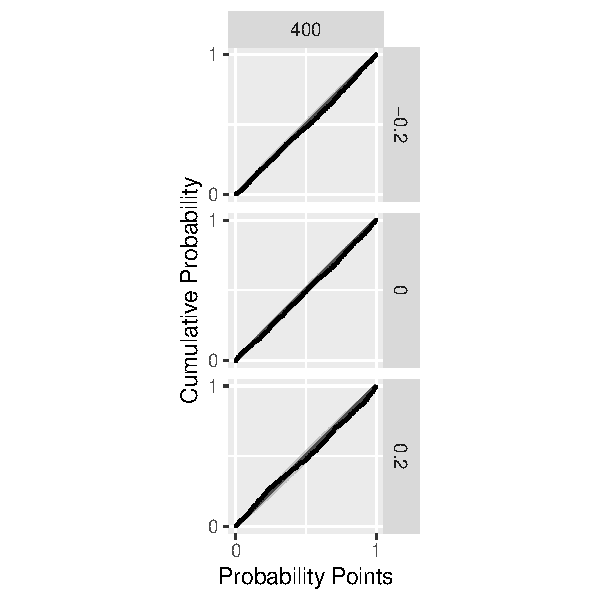
\includegraphics[scale=1]{figures/normal}
  \caption{A Q-Q plot of the p-values testing that a distribution
  generated from a $N(8,8)$ data generating process is normal.}
  \label{fig:normal}
\end{figure}

\begin{figure}[tbp]
  \centering
  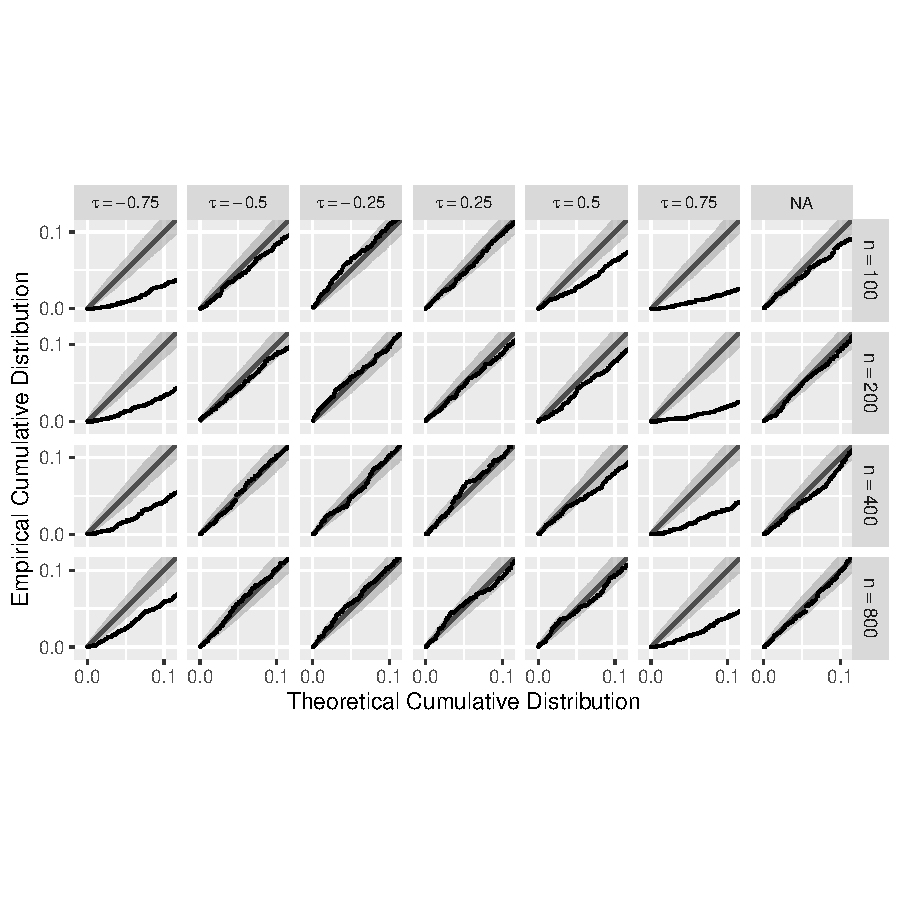
\includegraphics[scale=1]{figures/zoom_normal}
  \caption{A Q-Q plot of the p-values displayed in \ref{fig:normal} zoomed in to 
  probabilities between 0 and
  0.1}
  \label{fig:zoom_normal}
\end{figure}

\begin{figure}[tbp]
  \centering
  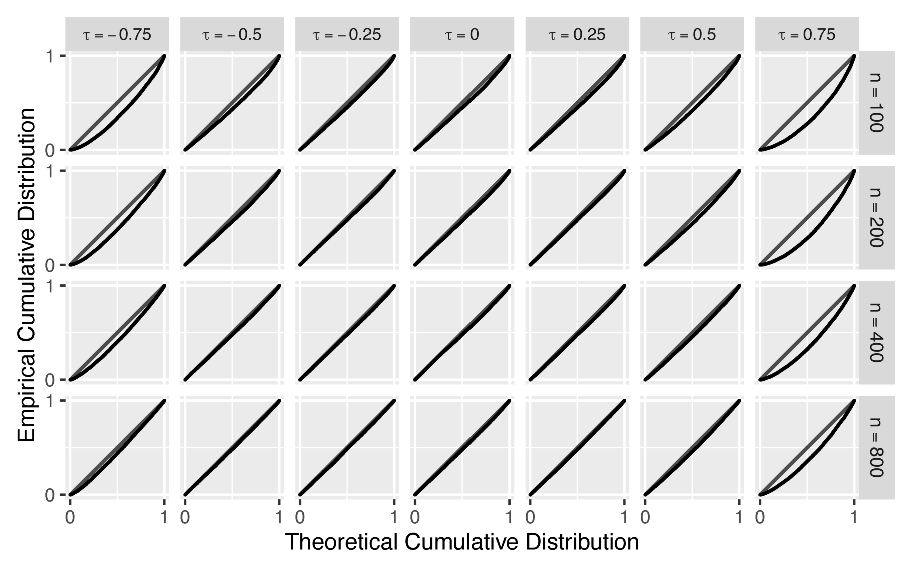
\includegraphics[scale=1]{figures/gamma}
  \caption{A Q-Q plot of the p-values testing that a distribution
  generated from a $\gamma(8,1)$ data generating process is gamma distributed.}
  \label{fig:gamma}
\end{figure}

\begin{figure}[tbp]
  \centering
  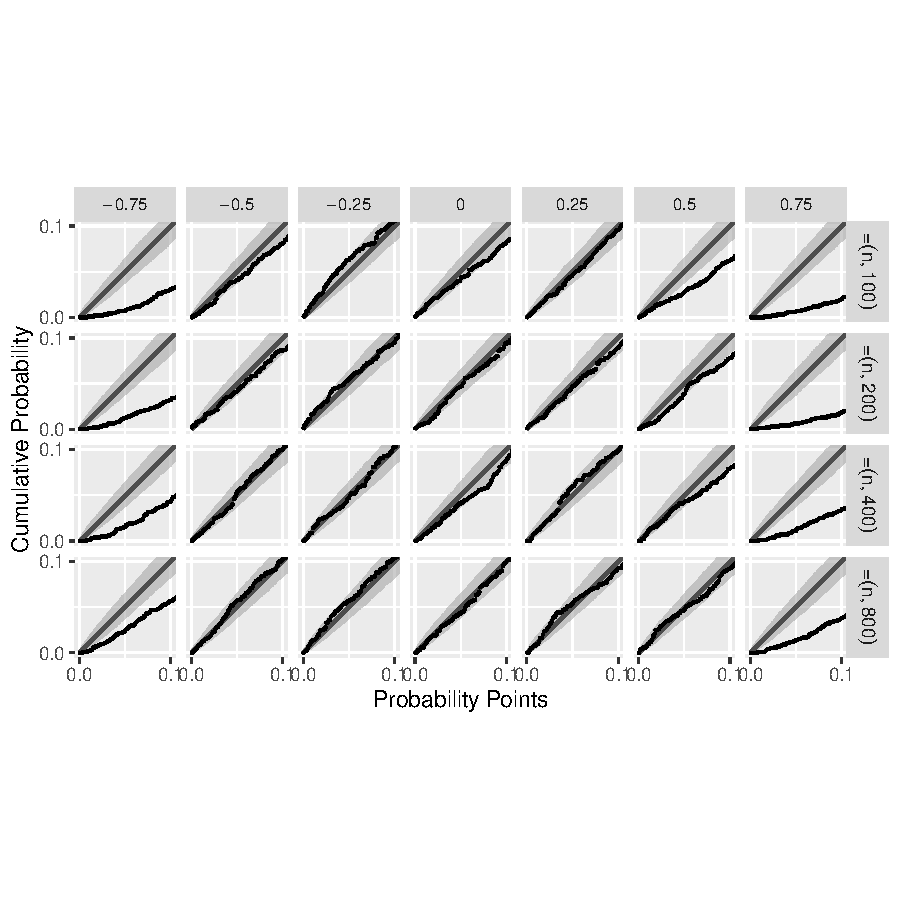
\includegraphics[scale=1]{figures/zoom_gamma}
  \caption{A Q-Q plot of the p-values displayed in \ref{fig:gamma} zoomed in to 
  probabilities between 0 and
  0.1}
  \label{fig:zoom_gamma}
\end{figure}


\paragraph{Power}
We must also evaluate if this method works when $H_0$ is false. We can use
the block bootstrap KS test to test if $X_t$ is generated from some other 
distribution $G$ with some unknown $\theta$. In this scenario, if the test is 
indeed powerful,
we would ideally want $\beta$, or the probability of rejection to be 1, but we
expect it to be generally high. Again, we must try the method with different
marginal distributions to ensure that it is robust.
We would then expect the distribution of p-values to be non-uniform, and the rate
of $\#P < \alpha$ to be high, meaning a higher density of low p-values.

If we can show that the test correctly fails to reject $H_0$ under the null
distribution, and correctly rejects $H_0$ for an alternate distribution, we can
state that the method works.

We can find the rate of rejection for  different values for the significance 
level $\alpha$. Additionally, we can construct a 95\% confidence interval for 
this rate. Below are rejection rates for $\phi = 0.2$ and $n = 800$, when
applied to the normal and gamma distributions using $\alpha =$ 0.01, 0.05, and 
0.10.

% latex table generated in R 4.3.0 by xtable 1.8-4 package
% Mon Apr 15 22:07:47 2024
\begin{table}[ht]
\centering
\caption{Rejection rates for test under true null hypothesis
                   when n = 100 for 
                   different values of AR(1) coefficient and for different 
                   significance levels. Lower and upper bounds are also 
                   included.} 
\label{table:rr_100}
\begin{tabular}{rllllrrr}
  \hline
 & $\phi$ & $n$ & distribution & $\alpha$ & lower bound & rejection rate & upper bound \\ 
  \hline
1 & -0.9238795 & 100 & normal & 0.01 & 0.04 & 0.05 & 0.07 \\ 
  2 & -0.9238795 & 100 & normal & 0.05 & 0.12 & 0.14 & 0.16 \\ 
  3 & -0.9238795 & 100 & normal & 0.1 & 0.21 & 0.24 & 0.27 \\ 
  4 & -0.9238795 & 100 & gamma & 0.01 & 0.04 & 0.06 & 0.07 \\ 
  5 & -0.9238795 & 100 & gamma & 0.05 & 0.12 & 0.14 & 0.17 \\ 
  6 & -0.9238795 & 100 & gamma & 0.1 & 0.21 & 0.24 & 0.27 \\ 
  7 & -0.7071068 & 100 & normal & 0.01 & 0.01 & 0.01 & 0.02 \\ 
  8 & -0.7071068 & 100 & normal & 0.05 & 0.05 & 0.06 & 0.08 \\ 
  9 & -0.7071068 & 100 & normal & 0.1 & 0.11 & 0.13 & 0.15 \\ 
  10 & -0.7071068 & 100 & gamma & 0.01 & 0.01 & 0.02 & 0.02 \\ 
  11 & -0.7071068 & 100 & gamma & 0.05 & 0.05 & 0.07 & 0.08 \\ 
  12 & -0.7071068 & 100 & gamma & 0.1 & 0.11 & 0.13 & 0.15 \\ 
  13 & -0.3826834 & 100 & normal & 0.01 & 0.00 & 0.01 & 0.01 \\ 
  14 & -0.3826834 & 100 & normal & 0.05 & 0.03 & 0.04 & 0.05 \\ 
  15 & -0.3826834 & 100 & normal & 0.1 & 0.07 & 0.09 & 0.11 \\ 
  16 & -0.3826834 & 100 & gamma & 0.01 & 0.00 & 0.01 & 0.01 \\ 
  17 & -0.3826834 & 100 & gamma & 0.05 & 0.03 & 0.04 & 0.05 \\ 
  18 & -0.3826834 & 100 & gamma & 0.1 & 0.08 & 0.09 & 0.11 \\ 
  19 & 0 & 100 & normal & 0.01 & 0.01 & 0.01 & 0.02 \\ 
  20 & 0 & 100 & normal & 0.05 & 0.05 & 0.06 & 0.07 \\ 
  21 & 0 & 100 & normal & 0.1 & 0.10 & 0.12 & 0.15 \\ 
  22 & 0 & 100 & gamma & 0.01 & 0.01 & 0.01 & 0.02 \\ 
  23 & 0 & 100 & gamma & 0.05 & 0.05 & 0.06 & 0.07 \\ 
  24 & 0 & 100 & gamma & 0.1 & 0.11 & 0.13 & 0.15 \\ 
  25 & 0.3826834 & 100 & normal & 0.01 & 0.01 & 0.01 & 0.02 \\ 
  26 & 0.3826834 & 100 & normal & 0.05 & 0.04 & 0.06 & 0.07 \\ 
  27 & 0.3826834 & 100 & normal & 0.1 & 0.09 & 0.10 & 0.12 \\ 
  28 & 0.3826834 & 100 & gamma & 0.01 & 0.01 & 0.01 & 0.02 \\ 
  29 & 0.3826834 & 100 & gamma & 0.05 & 0.04 & 0.06 & 0.07 \\ 
  30 & 0.3826834 & 100 & gamma & 0.1 & 0.09 & 0.10 & 0.12 \\ 
  31 & 0.7071068 & 100 & normal & 0.01 & 0.01 & 0.01 & 0.02 \\ 
  32 & 0.7071068 & 100 & normal & 0.05 & 0.07 & 0.09 & 0.10 \\ 
  33 & 0.7071068 & 100 & normal & 0.1 & 0.13 & 0.15 & 0.18 \\ 
  34 & 0.7071068 & 100 & gamma & 0.01 & 0.01 & 0.02 & 0.03 \\ 
  35 & 0.7071068 & 100 & gamma & 0.05 & 0.07 & 0.09 & 0.10 \\ 
  36 & 0.7071068 & 100 & gamma & 0.1 & 0.13 & 0.15 & 0.17 \\ 
  37 & 0.9238795 & 100 & normal & 0.01 & 0.04 & 0.06 & 0.07 \\ 
  38 & 0.9238795 & 100 & normal & 0.05 & 0.16 & 0.18 & 0.20 \\ 
  39 & 0.9238795 & 100 & normal & 0.1 & 0.24 & 0.27 & 0.30 \\ 
  40 & 0.9238795 & 100 & gamma & 0.01 & 0.05 & 0.07 & 0.08 \\ 
  41 & 0.9238795 & 100 & gamma & 0.05 & 0.16 & 0.18 & 0.20 \\ 
  42 & 0.9238795 & 100 & gamma & 0.1 & 0.25 & 0.27 & 0.30 \\ 
   \hline
\end{tabular}
\end{table}



From \ref{table:rr_100}, we can see that when $n = 100$, the rejection rate may 
be quite low, especially for lower values of $\alpha$. From \ref{table:rr_200}, 
the rejection rates are a little higher for $n = 200$, but they may still be 
drop below 50\% is the $\alpha = 0.1$. Once $n$ reaches 400, we can observe 
from \ref{table:rr_400} that the rejection rate
is consistently above 50\%. For larger sample sizes, the rejection rate is 
consistently above 90\%. We can also
observe that the rejection rate is higher for the $\gamma(8, 1)$ sample than for 
the $N(8, 8)$ As the strength of the temporal dependence increases, the 
rejection rate decreases, and the rejection
rate appears to be slightly higher for negative temporal dependence versus 
positive temporal dependence values of the same strength.

% latex table generated in R 4.3.0 by xtable 1.8-4 package
% Fri Dec  8 15:41:08 2023
\begin{table}[ht]
\centering
\begin{tabular}{rlllllll}
  \hline
 & phi & n & distribution & alpha & lower bound & rejection rate & upper bound \\ 
  \hline
1 & -0.4 & 200 & normal & 0.01 & 0.376963148552451 & 0.407355888539157 & 0.437748628525863 \\ 
  2 & -0.4 & 200 & normal & 0.05 & 0.666785180010044 & 0.695249955336831 & 0.723714730663618 \\ 
  3 & -0.4 & 200 & normal & 0.1 & 0.769913574238833 & 0.794867279488276 & 0.819820984737718 \\ 
  4 & -0.4 & 200 & gamma & 0.01 & 0.422385886474774 & 0.453179857648821 & 0.483973828822868 \\ 
  5 & -0.4 & 200 & gamma & 0.05 & 0.703698575421144 & 0.731112192031351 & 0.758525808641559 \\ 
  6 & -0.4 & 200 & gamma & 0.1 & 0.821253161260159 & 0.843679768322483 & 0.866106375384808 \\ 
  7 & -0.2 & 200 & normal & 0.01 & 0.362210225188365 & 0.39241328991644 & 0.422616354644515 \\ 
  8 & -0.2 & 200 & normal & 0.05 & 0.63923606946991 & 0.668353277815941 & 0.697470486161972 \\ 
  9 & -0.2 & 200 & normal & 0.1 & 0.774081035351865 & 0.798851972454333 & 0.823622909556802 \\ 
  10 & -0.2 & 200 & gamma & 0.01 & 0.416446007701489 & 0.447202818199734 & 0.47795962869798 \\ 
  11 & -0.2 & 200 & gamma & 0.05 & 0.721208085064392 & 0.748047137137097 & 0.774886189209802 \\ 
  12 & -0.2 & 200 & gamma & 0.1 & 0.828644950702635 & 0.850652981013085 & 0.872661011323534 \\ 
  13 & 0 & 200 & normal & 0.01 & 0.332794412867473 & 0.362528092671007 & 0.39226177247454 \\ 
  14 & 0 & 200 & normal & 0.05 & 0.644329419483164 & 0.673334144023513 & 0.702338868563863 \\ 
  15 & 0 & 200 & normal & 0.1 & 0.769913574238833 & 0.794867279488276 & 0.819820984737718 \\ 
  16 & 0 & 200 & gamma & 0.01 & 0.417435674584357 & 0.448198991441249 & 0.478962308298141 \\ 
  17 & 0 & 200 & gamma & 0.05 & 0.698558600564729 & 0.726131325823779 & 0.753704051082829 \\ 
  18 & 0 & 200 & gamma & 0.1 & 0.801267303732901 & 0.824752476733709 & 0.848237649734517 \\ 
  19 & 0.2 & 200 & normal & 0.01 & 0.334751650912775 & 0.364520439154035 & 0.394289227395296 \\ 
  20 & 0.2 & 200 & normal & 0.05 & 0.613823930034022 & 0.64344894677808 & 0.673073963522138 \\ 
  21 & 0.2 & 200 & normal & 0.1 & 0.739807130220676 & 0.765978255484357 & 0.792149380748038 \\ 
  22 & 0.2 & 200 & gamma & 0.01 & 0.406556246868357 & 0.43724108578459 & 0.467925924700823 \\ 
  23 & 0.2 & 200 & gamma & 0.05 & 0.696503832704027 & 0.72413897934075 & 0.751774125977474 \\ 
  24 & 0.2 & 200 & gamma & 0.1 & 0.809669197162261 & 0.832721862665825 & 0.855774528169388 \\ 
  25 & 0.4 & 200 & normal & 0.01 & 0.299744126407305 & 0.328946560348041 & 0.358148994288778 \\ 
  26 & 0.4 & 200 & normal & 0.05 & 0.596715074425386 & 0.626780784683216 & 0.656846494941047 \\ 
  27 & 0.4 & 200 & normal & 0.1 & 0.73409479567292 & 0.760604946293278 & 0.787115096913636 \\ 
  28 & 0.4 & 200 & gamma & 0.01 & 0.357023355418913 & 0.387305969170474 & 0.417588582922036 \\ 
  29 & 0.4 & 200 & gamma & 0.05 & 0.653180037970102 & 0.682121603394144 & 0.711063168818186 \\ 
  30 & 0.4 & 200 & gamma & 0.1 & 0.788712564776464 & 0.8129271748927 & 0.837141785008937 \\ 
   \hline
\end{tabular}
\caption{Rejection rates for test when n = 200 for 
                   different values of AR(1) coefficient and for different 
                   significance levels. Lower and upper bounds are also 
                   included.} 
\label{table:rr_200}
\end{table}




% latex table generated in R 4.3.0 by xtable 1.8-4 package
% Sun Jan 21 19:49:53 2024
\begin{table}[ht]
\centering
\caption{Rejection rates for test when n = 400 for 
                   different values of AR(1) coefficient and for different 
                   significance levels. Lower and upper bounds are also 
                   included.} 
\label{table:rr_400}
\begin{tabular}{rllllrrr}
  \hline
 & phi & n & distribution & alpha & lower bound & rejection rate & upper bound \\ 
  \hline
1 & -0.4 & 400 & normal & 0.05 & 0.95 & 0.96 & 0.97 \\ 
  2 & -0.4 & 400 & gamma & 0.05 & 0.94 & 0.96 & 0.97 \\ 
  3 & -0.2 & 400 & normal & 0.05 & 0.94 & 0.95 & 0.97 \\ 
  4 & -0.2 & 400 & gamma & 0.05 & 0.94 & 0.95 & 0.96 \\ 
  5 & 0 & 400 & normal & 0.05 & 0.93 & 0.95 & 0.96 \\ 
  6 & 0 & 400 & gamma & 0.05 & 0.93 & 0.94 & 0.96 \\ 
  7 & 0.2 & 400 & normal & 0.05 & 0.94 & 0.95 & 0.96 \\ 
  8 & 0.2 & 400 & gamma & 0.05 & 0.93 & 0.95 & 0.96 \\ 
  9 & 0.4 & 400 & normal & 0.05 & 0.92 & 0.93 & 0.95 \\ 
  10 & 0.4 & 400 & gamma & 0.05 & 0.92 & 0.94 & 0.95 \\ 
   \hline
\end{tabular}
\end{table}



% latex table generated in R 4.3.0 by xtable 1.8-4 package
% Mon Apr 15 22:07:47 2024
\begin{table}[ht]
\centering
\caption{Rejection rates for test under true null hypothesis
                   when n = 800 for 
                   different values of AR(1) coefficient and for different 
                   significance levels. Lower and upper bounds are also 
                   included.} 
\label{table:rr_800}
\begin{tabular}{rllllrrr}
  \hline
 & $\phi$ & $n$ & distribution & $\alpha$ & lower bound & rejection rate & upper bound \\ 
  \hline
1 & -0.9238795 & 800 & normal & 0.01 & 0.01 & 0.03 & 0.03 \\ 
  2 & -0.9238795 & 800 & normal & 0.05 & 0.07 & 0.09 & 0.11 \\ 
  3 & -0.9238795 & 800 & normal & 0.1 & 0.14 & 0.17 & 0.19 \\ 
  4 & -0.9238795 & 800 & gamma & 0.01 & 0.02 & 0.03 & 0.04 \\ 
  5 & -0.9238795 & 800 & gamma & 0.05 & 0.07 & 0.09 & 0.11 \\ 
  6 & -0.9238795 & 800 & gamma & 0.1 & 0.15 & 0.17 & 0.19 \\ 
  7 & -0.7071068 & 800 & normal & 0.01 & 0.01 & 0.01 & 0.02 \\ 
  8 & -0.7071068 & 800 & normal & 0.05 & 0.03 & 0.04 & 0.06 \\ 
  9 & -0.7071068 & 800 & normal & 0.1 & 0.08 & 0.10 & 0.12 \\ 
  10 & -0.7071068 & 800 & gamma & 0.01 & 0.01 & 0.01 & 0.02 \\ 
  11 & -0.7071068 & 800 & gamma & 0.05 & 0.03 & 0.04 & 0.06 \\ 
  12 & -0.7071068 & 800 & gamma & 0.1 & 0.08 & 0.10 & 0.12 \\ 
  13 & -0.3826834 & 800 & normal & 0.01 & 0.00 & 0.01 & 0.02 \\ 
  14 & -0.3826834 & 800 & normal & 0.05 & 0.03 & 0.04 & 0.05 \\ 
  15 & -0.3826834 & 800 & normal & 0.1 & 0.08 & 0.10 & 0.12 \\ 
  16 & -0.3826834 & 800 & gamma & 0.01 & 0.00 & 0.01 & 0.01 \\ 
  17 & -0.3826834 & 800 & gamma & 0.05 & 0.03 & 0.04 & 0.06 \\ 
  18 & -0.3826834 & 800 & gamma & 0.1 & 0.08 & 0.10 & 0.11 \\ 
  19 & 0 & 800 & normal & 0.01 & 0.01 & 0.01 & 0.02 \\ 
  20 & 0 & 800 & normal & 0.05 & 0.04 & 0.06 & 0.07 \\ 
  21 & 0 & 800 & normal & 0.1 & 0.09 & 0.10 & 0.12 \\ 
  22 & 0 & 800 & gamma & 0.01 & 0.01 & 0.01 & 0.02 \\ 
  23 & 0 & 800 & gamma & 0.05 & 0.04 & 0.06 & 0.07 \\ 
  24 & 0 & 800 & gamma & 0.1 & 0.08 & 0.10 & 0.12 \\ 
  25 & 0.3826834 & 800 & normal & 0.01 & 0.01 & 0.01 & 0.02 \\ 
  26 & 0.3826834 & 800 & normal & 0.05 & 0.03 & 0.04 & 0.06 \\ 
  27 & 0.3826834 & 800 & normal & 0.1 & 0.09 & 0.11 & 0.13 \\ 
  28 & 0.3826834 & 800 & gamma & 0.01 & 0.01 & 0.01 & 0.02 \\ 
  29 & 0.3826834 & 800 & gamma & 0.05 & 0.03 & 0.05 & 0.06 \\ 
  30 & 0.3826834 & 800 & gamma & 0.1 & 0.09 & 0.11 & 0.13 \\ 
  31 & 0.7071068 & 800 & normal & 0.01 & 0.01 & 0.01 & 0.02 \\ 
  32 & 0.7071068 & 800 & normal & 0.05 & 0.04 & 0.06 & 0.07 \\ 
  33 & 0.7071068 & 800 & normal & 0.1 & 0.09 & 0.11 & 0.13 \\ 
  34 & 0.7071068 & 800 & gamma & 0.01 & 0.01 & 0.01 & 0.02 \\ 
  35 & 0.7071068 & 800 & gamma & 0.05 & 0.04 & 0.05 & 0.07 \\ 
  36 & 0.7071068 & 800 & gamma & 0.1 & 0.09 & 0.11 & 0.13 \\ 
  37 & 0.9238795 & 800 & normal & 0.01 & 0.03 & 0.04 & 0.05 \\ 
  38 & 0.9238795 & 800 & normal & 0.05 & 0.11 & 0.13 & 0.15 \\ 
  39 & 0.9238795 & 800 & normal & 0.1 & 0.17 & 0.20 & 0.22 \\ 
  40 & 0.9238795 & 800 & gamma & 0.01 & 0.03 & 0.04 & 0.05 \\ 
  41 & 0.9238795 & 800 & gamma & 0.05 & 0.10 & 0.12 & 0.14 \\ 
  42 & 0.9238795 & 800 & gamma & 0.1 & 0.17 & 0.20 & 0.22 \\ 
   \hline
\end{tabular}
\end{table}



% latex table generated in R 4.3.0 by xtable 1.8-4 package
% Sun Dec  3 13:33:51 2023
\begin{table}[ht]
\centering
\begin{tabular}{rlllllll}
  \hline
 & phi & n & distribution & alpha & lower bound & rejection rate & upper bound \\ 
  \hline
1 & -0.4 & 1600 & normal & 0.01 & 0.996173241514445 & 0.998086620757222 & 1 \\ 
  2 & -0.4 & 1600 & normal & 0.05 & 0.996173241514445 & 0.998086620757222 & 1 \\ 
  3 & -0.4 & 1600 & normal & 0.1 & 0.996173241514445 & 0.998086620757222 & 1 \\ 
  4 & -0.4 & 1600 & gamma & 0.01 & 0.996173241514445 & 0.998086620757222 & 1 \\ 
  5 & -0.4 & 1600 & gamma & 0.05 & 0.996173241514445 & 0.998086620757222 & 1 \\ 
  6 & -0.4 & 1600 & gamma & 0.1 & 0.996173241514445 & 0.998086620757222 & 1 \\ 
  7 & -0.2 & 1600 & normal & 0.01 & 0.996173241514445 & 0.998086620757222 & 1 \\ 
  8 & -0.2 & 1600 & normal & 0.05 & 0.996173241514445 & 0.998086620757222 & 1 \\ 
  9 & -0.2 & 1600 & normal & 0.1 & 0.996173241514445 & 0.998086620757222 & 1 \\ 
  10 & -0.2 & 1600 & gamma & 0.01 & 0.996173241514445 & 0.998086620757222 & 1 \\ 
  11 & -0.2 & 1600 & gamma & 0.05 & 0.996173241514445 & 0.998086620757222 & 1 \\ 
  12 & -0.2 & 1600 & gamma & 0.1 & 0.996173241514445 & 0.998086620757222 & 1 \\ 
  13 & 0 & 1600 & normal & 0.01 & 0.996173241514445 & 0.998086620757222 & 1 \\ 
  14 & 0 & 1600 & normal & 0.05 & 0.996173241514445 & 0.998086620757222 & 1 \\ 
  15 & 0 & 1600 & normal & 0.1 & 0.996173241514445 & 0.998086620757222 & 1 \\ 
  16 & 0 & 1600 & gamma & 0.01 & 0.996173241514445 & 0.998086620757222 & 1 \\ 
  17 & 0 & 1600 & gamma & 0.05 & 0.996173241514445 & 0.998086620757222 & 1 \\ 
  18 & 0 & 1600 & gamma & 0.1 & 0.996173241514445 & 0.998086620757222 & 1 \\ 
  19 & 0.2 & 1600 & normal & 0.01 & 0.996173241514445 & 0.998086620757222 & 1 \\ 
  20 & 0.2 & 1600 & normal & 0.05 & 0.996173241514445 & 0.998086620757222 & 1 \\ 
  21 & 0.2 & 1600 & normal & 0.1 & 0.996173241514445 & 0.998086620757222 & 1 \\ 
  22 & 0.2 & 1600 & gamma & 0.01 & 0.996173241514445 & 0.998086620757222 & 1 \\ 
  23 & 0.2 & 1600 & gamma & 0.05 & 0.996173241514445 & 0.998086620757222 & 1 \\ 
  24 & 0.2 & 1600 & gamma & 0.1 & 0.996173241514445 & 0.998086620757222 & 1 \\ 
  25 & 0.4 & 1600 & normal & 0.01 & 0.996134736796699 & 0.99806736839835 & 1 \\ 
  26 & 0.4 & 1600 & normal & 0.05 & 0.996134736796699 & 0.99806736839835 & 1 \\ 
  27 & 0.4 & 1600 & normal & 0.1 & 0.996134736796699 & 0.99806736839835 & 1 \\ 
  28 & 0.4 & 1600 & gamma & 0.01 & 0.996134736796699 & 0.99806736839835 & 1 \\ 
  29 & 0.4 & 1600 & gamma & 0.05 & 0.996134736796699 & 0.99806736839835 & 1 \\ 
  30 & 0.4 & 1600 & gamma & 0.1 & 0.996134736796699 & 0.99806736839835 & 1 \\ 
   \hline
\end{tabular}
\caption{Rejection rates for test when n = 1600 for 
                   different values of AR(1) coefficient and for different 
                   significance levels. Lower and upper bounds are also 
                   included.} 
\label{rr_1600}
\end{table}



% latex table generated in R 4.3.0 by xtable 1.8-4 package
% Wed Dec 13 23:00:44 2023
\begin{table}[ht]
\centering
\caption{Rejection rates for test when n = 3200 for 
                   different values of AR(1) coefficient and for different 
                   significance levels. Lower and upper bounds are also 
                   included.} 
\label{table:rr_3200}
\begin{tabular}{rlllllll}
  \hline
 & phi & n & distribution & alpha & lower bound & rejection rate & upper bound \\ 
  \hline
1 & -0.4 & 3200 & normal & 0.01 & 0.996173241514445 & 0.998086620757222 & 1 \\ 
  2 & -0.4 & 3200 & normal & 0.05 & 0.996173241514445 & 0.998086620757222 & 1 \\ 
  3 & -0.4 & 3200 & normal & 0.1 & 0.996173241514445 & 0.998086620757222 & 1 \\ 
  4 & -0.4 & 3200 & gamma & 0.01 & 0.996173241514445 & 0.998086620757222 & 1 \\ 
  5 & -0.4 & 3200 & gamma & 0.05 & 0.996173241514445 & 0.998086620757222 & 1 \\ 
  6 & -0.4 & 3200 & gamma & 0.1 & 0.996173241514445 & 0.998086620757222 & 1 \\ 
  7 & -0.2 & 3200 & normal & 0.01 & 0.996173241514445 & 0.998086620757222 & 1 \\ 
  8 & -0.2 & 3200 & normal & 0.05 & 0.996173241514445 & 0.998086620757222 & 1 \\ 
  9 & -0.2 & 3200 & normal & 0.1 & 0.996173241514445 & 0.998086620757222 & 1 \\ 
  10 & -0.2 & 3200 & gamma & 0.01 & 0.996173241514445 & 0.998086620757222 & 1 \\ 
  11 & -0.2 & 3200 & gamma & 0.05 & 0.996173241514445 & 0.998086620757222 & 1 \\ 
  12 & -0.2 & 3200 & gamma & 0.1 & 0.996173241514445 & 0.998086620757222 & 1 \\ 
  13 & 0 & 3200 & normal & 0.01 & 0.996173241514445 & 0.998086620757222 & 1 \\ 
  14 & 0 & 3200 & normal & 0.05 & 0.996173241514445 & 0.998086620757222 & 1 \\ 
  15 & 0 & 3200 & normal & 0.1 & 0.996173241514445 & 0.998086620757222 & 1 \\ 
  16 & 0 & 3200 & gamma & 0.01 & 0.996173241514445 & 0.998086620757222 & 1 \\ 
  17 & 0 & 3200 & gamma & 0.05 & 0.996173241514445 & 0.998086620757222 & 1 \\ 
  18 & 0 & 3200 & gamma & 0.1 & 0.996173241514445 & 0.998086620757222 & 1 \\ 
  19 & 0.2 & 3200 & normal & 0.01 & 0.996134736796699 & 0.99806736839835 & 1 \\ 
  20 & 0.2 & 3200 & normal & 0.05 & 0.996134736796699 & 0.99806736839835 & 1 \\ 
  21 & 0.2 & 3200 & normal & 0.1 & 0.996134736796699 & 0.99806736839835 & 1 \\ 
  22 & 0.2 & 3200 & gamma & 0.01 & 0.996134736796699 & 0.99806736839835 & 1 \\ 
  23 & 0.2 & 3200 & gamma & 0.05 & 0.996134736796699 & 0.99806736839835 & 1 \\ 
  24 & 0.2 & 3200 & gamma & 0.1 & 0.996134736796699 & 0.99806736839835 & 1 \\ 
  25 & 0.4 & 3200 & normal & 0.01 & 0.996134736796699 & 0.99806736839835 & 1 \\ 
  26 & 0.4 & 3200 & normal & 0.05 & 0.996134736796699 & 0.99806736839835 & 1 \\ 
  27 & 0.4 & 3200 & normal & 0.1 & 0.996134736796699 & 0.99806736839835 & 1 \\ 
  28 & 0.4 & 3200 & gamma & 0.01 & 0.996134736796699 & 0.99806736839835 & 1 \\ 
  29 & 0.4 & 3200 & gamma & 0.05 & 0.996134736796699 & 0.99806736839835 & 1 \\ 
  30 & 0.4 & 3200 & gamma & 0.1 & 0.996134736796699 & 0.99806736839835 & 1 \\ 
   \hline
\end{tabular}
\end{table}



As shown in the above table, the rejection rates for these settings are very 
high (almost 1), indicating that the test is very powerful for these settings.

\section{Real Data Analysis}



\jy{Find some real time series to test for their marginal distributions. Open
  data, for example, temperatures or stock returns or ...}

\subsection{Precipitation in Mansfield Connecticut}
Annual maximums of hourly precipitation in inches time series data were 
retrieved 
from the Chicago Midway International Airport, New York LaGuardia International 
Airport,
and Los Angeles International Airport stations from the 
National Oceanic and Atmospheric Administration. These stations were selected 
from places of importance in the three largest American cities. LaGuardia and
Midway were chosen over John F. Kennedy and O'Hare as more data was available
from these stations. The data is from
May 1st of 1948 to January 1st of 2014. To confirm that our method works, we 
used it to test that
the precipitation time series from each of these locations followed the 
Generalized Extreme Value (GEV) distribution. 

% latex table generated in R 4.3.0 by xtable 1.8-4 package
% Sun Feb 25 12:46:58 2024
\begin{table}[ht]
\centering
\caption{P-values for testing that annual maximums of hourly 
            precipitation from the three airports follows the GEV distribution.} 
\label{table:precipitation}
\begin{tabular}{rrrr}
  \hline
 & block & basic & param \\ 
  \hline
MDW & 0.16 & 0.21 & 0.08 \\ 
  LGA & 0.44 & 0.55 & 0.48 \\ 
  LAX & 0.28 & 0.36 & 0.34 \\ 
   \hline
\end{tabular}
\end{table}


%\mc{https://hdsc.nws.noaa.gov/pfds/pfds_map_cont.html?bkmrk=ct}

Using a significance level as high as .10 still results in a failed rejection
of the null hypothesis that all three time series follow the GEV distribution.

\subsection{Microsoft Stock Returns}

%\mc{https://www.nasdaq.com/market-activity/stocks/msft/historical}

We expect the distribution of Microsoft stock returns to have a slightly
heavier tail than the normal distribution. We can test that it is normally
distributed (which we expect to reject).  While we 
could choose to estimate a fited value of the degrees of freedom parameter as
part of our method, it is very difficult to do so. Therefore, we can try testing 
if it follows
the $t$ distribution with increasingly smaller degrees of freedoms.

% latex table generated in R 4.3.0 by xtable 1.8-4 package
% Mon Feb  5 18:44:34 2024
\begin{table}[ht]
\centering
\caption{P-values for Microsoft stock return data using different durations
  and different degrees of freedom for Student's t distribution.} 
\label{table:microsoft}
\begin{tabular}{rlrrrrrrrrr}
  \hline
 & Duration & Normal & t..v...30 & t..v...20 & t..v...10 & t..v...7 & t..v...5 & t..v...4 & t..v...3 & t..v...2 \\ 
  \hline
1 & 5 Years & 0.00 & 0.00 & 0.00 & 0.00 & 0.00 & 0.01 & 0.10 & 0.20 & 0.00 \\ 
  2 & 4 Years & 0.00 & 0.00 & 0.00 & 0.00 & 0.00 & 0.03 & 0.12 & 0.08 & 0.00 \\ 
  3 & 3 Years & 0.00 & 0.00 & 0.00 & 0.00 & 0.01 & 0.07 & 0.27 & 0.27 & 0.01 \\ 
  4 & 2 Years & 0.00 & 0.00 & 0.00 & 0.01 & 0.01 & 0.01 & 0.01 & 0.02 & 0.01 \\ 
  5 & 1.5 Years & 0.01 & 0.02 & 0.03 & 0.07 & 0.07 & 0.07 & 0.07 & 0.10 & 0.23 \\ 
  6 & 1 Year & 0.56 & 0.59 & 0.61 & 0.65 & 0.72 & 0.57 & 0.39 & 0.22 & 0.09 \\ 
   \hline
\end{tabular}
\end{table}



F

\section{Concluding Remarks}
\label{sec:conclusion}

Using simulation, we have shown that given a large enough sample of a time 
series, the block 
bootstrap KS test can appropriately fail to reject the null hypothesis when the
series follows the null distribution. In addition, when the marginal
distribution is not
the one hypothesized, the test is powerful. It requires a larger sample size 
than basic bootstrap to avoid either type I or type II errors. Unsurprisingly,
the method performs better as the temporal dependence gets weaker. We have also 
demonstrated possible applications of this method to precipitation and 
stock return data. This method can be used for any study where the goal is
to see if a time series follows a hypothesized distribution and the parameters
are unknown or unspecified. 





\bibliographystyle{chicago}
\bibliography{citations}


\end{document}
%%% LocalWords: nonparametric semiparametric autocorrelation ARMA
%%% Local Variables:
%%% mode: latex
%%% TeX-master: t
%%% ispell-personal-dictionary: ".aspell.en.pws"
%%% fill-column: 80
%%% eval: (auto-fill-mode 1)
%%% End: